\chapter{Grundlagen}
\label{cha:Grundlagen}

%
% Einleitung zuletzt schreiben. Roter Faden?
% 
%Was ist testgetriebene Entwicklung? Welche Besonderheiten ergeben sich im Zusammenhang mit der Entwicklung einer JavaScript-App und der SAP-Infrastruktur?
%
%
%SAP Mobile Entwicklungen, Architekturen, Open Source, neues Backend

\autsection{Was ist testgetriebene Entwicklung?}{Mattfeld}

Beispielhaft zeigt \autoref{fig:tdd-circle} den Kern der Methode -- Die Entwicklung erfolgt In 3 Schritten:

\begin{description}
	\item[Rote Phase:] Eine noch nicht implementierte Funktion wird durch einen Test geprüft. Dieser schlägt fehl -- Ist also \textit{rot}.
	\item[Grüne Phase:] Die Funktion wird implementiert, der Testlauf ist erfolgreich und der Teststatus entsprechend \textit{grün}.
	\item[Refaktorisierung:] Der Quellcode wird verbessert, Redundanzen entfernt.
\end{description}
% Kein Absatz -> Kein Einzug
Diese Schritte wiederholen sich in einer Endlosschleife während der gesamten Entwicklungszeit. Im Unterschied zu klassischen Herangehensweisen werden zuerst Tests geschrieben und erst danach Funktionalitäten implementiert.

\begin{figure}
	\centering
	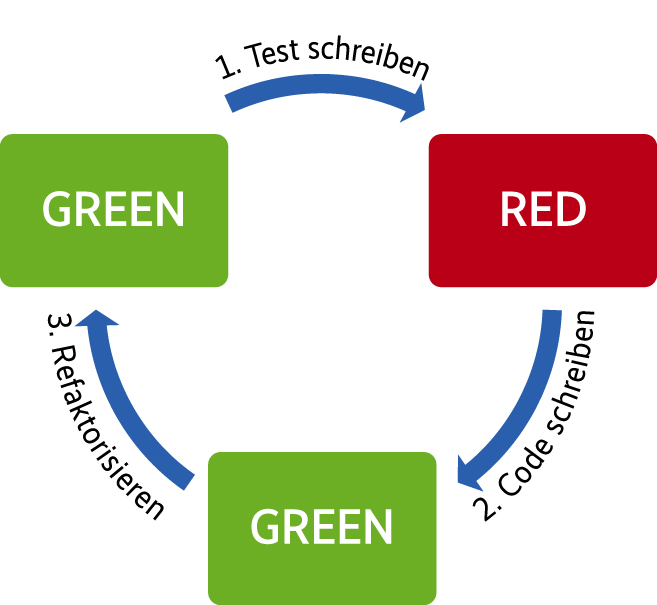
\includegraphics[width=.5\textwidth]{tdd-circle} 
	\caption[TDD-Entwicklungskreislauf]{TDD-Entwicklungskreislauf aus \cite{heise2013}.}
	\label{fig:tdd-circle}
\end{figure}

\subsection{Vorteile der Methode}
Laut Beschreibung scheint \ac{TDD} gleichbedeutend mit höherem Aufwand durch den zusätzlichen oder zumindest umfangreicheren Testumfang. Wo ist der Mehrwert? 

\ZB nach \autoref{tab:maintenance-cost} liegt der Anteil an Wartungskosten innerhalb eines Softwareprojektes bei mindestens 80\,\% -- Tendenz weiter steigend. Gemeint sind Aufwände für Erweiterungen und Fehlerbehebungen. Die Hauptaufgabe der Methode \ac{TDD} ist folglich die langfristige Reduzierung des Wartungsaufwands und damit eine Kosteneinsparung.

\begin{table}
	\centering
\begin{tabular}{ccc}
	\toprule Referenz & Zeitraum & \%\,Wartung \\ 
	\midrule Pigoski (1997) & 1985-1989 & 75\,\% \\ 
			 Frazer (1992) & 1990 & 80\,\% \\ 
			 Pigoski (1997) & 1990s & 90\,\% \\ 
	\bottomrule 
\end{tabular} 
\caption{Anteil der Wartungskosten in Softwareprojekten nach \cite[S.\,229]{PoloPiattiniRuiz2002}.}
\label{tab:maintenance-cost}
\end{table} 

\subsubsection{Keine Schnellstarts}
Klassische Entwicklungsmethoden verleiten zu Schnellstarts -- Erst programmieren, dann die Anforderungen verfeinern und nachbessern. Der Zwang erst Tests zu schreiben, führt fast zwangsläufig zu einer intensiveren Analysephase, da die zu lösenden Probleme erst verstanden und zerlegt werden müssen. Die Entwicklung wird auf die richtigen Funktionalitäten fokussiert. Daraus ergeben sich weitere Vorteile in Bezug auf Code-Umfang und -Qualität.

\subsubsection{Weniger Code -- Besserer Code}
Durch die Zerlegung in testbare Teilprobleme wird von Anfang an eine modulare Software-Architektur aufgebaut. Die Abhängigkeiten sind klar definiert, die Anwendung kann leicht erweitert oder korrigiert werden.

Im Optimalfall entsteht nur Code, der auch getestet wird. Jede Funktion muss ein vorher festgelegtes Teilproblem lösen und einen Test erfüllen. Dieses Vorgehen verhindert die Entstehung von unnötigem Code und ermöglicht die Konzentration auf das Wesentliche. Die Refactoring-Phase sorgt für die Eliminierung von Code-Duplikaten. Jede Aufgabe wird nur einmal gelöst.

\subsubsection{Jeder Fehler nur einmal}
Die stetige Überarbeitung sorgt für geringe \textit{technische Schulden} im Code \cite[S.\ 13]{Springer2015}. Weiterführend ändert sich auch der Umgang mit Bugs: Für jeden festgestellten Fehler wird ein eigener Testfall geschrieben. Erst danach beginnt die Korrektur im Code. Hierdurch werden automatische Regressionstests möglich -- Jeder Fehler wird nur einmal begangen.

All dies führt zu einer wartungsfreundlicheren Applikation, die während ihres Lebenszyklus, trotz höherem Initialaufwands, im Vergleich Kosten einsparen kann. Was ist nötig um \ac{TDD} erfolgreich einzusetzen?

\subsection{Wege zum Erfolg}
\ac{TDD} erfordert viel Umgewöhnung -- Einen Test für nicht-existierende Funktionalitäten zu schreiben erscheint ungewöhnlich. Um die Methode trotzdem zum Erfolg zu führen helfen:

\begin{itemize}
	\item Hochintegrierte Entwicklungsumgebungen
	\item Automatisierte Tests
	\item \ac{CI}
	\item Transparenz
	\item Übung und Schulungen
\end{itemize}
%
Im Folgenden die wichtigsten Richtlinien, die wir für dieses Projekt aus \ac{TDD}-Best-Practices \cite[S.\ 99]{Seidl2012} übernommen haben.

\subsubsection{Unterstützende Entwicklungsumgebung}
Auch wenn einigen Programmierern  ein einfacher Texteditor und die Kommandozeile genügen (zum Beispiel \cite{Roden2015}) -- Wichtig sind möglichst wenig Kontextwechsel während der Entwicklung, und damit eine hochintegrierte Entwicklungsumgebung. Das Werkzeug soll in den Hintergrund rücken und \ac{TDD} aktiv unterstützen.

Konkret benötigen wir Syntax-Hervorhebung der genutzten Sprache (JavaScript), die Integration von statischen Code-Analysen, Unit-Tests, Test-Treibern, Build-Systemen, Versionsverwaltungen, Verwaltung von Abhängigkeiten und einigen weiteren Funktionen, die wir in \autoref{sec:auswahl_ide} erläutern.

\subsubsection{Testfallanforderungen}
Die Codequalität eines Tests muss grundsätzlich den gleichen Ansprüchen genügen, wie die des Hauptcodes. Auch die Tests werden schließlich während des Softwarelebenzykluses immer wieder gewartet und erweitert. Lesbarkeit und Modularität sind entscheidende Erfolgsfaktoren. Im Optimalfall sind die Tests sprechend und selbsterklärend formuliert.

Eine Folge der Modularität ist Unabhängigkeit. Ein Testfall sollte nicht vom Erfolg eines anderen Testfalls abhängen, sondern allein lauffähig sein. Während eines Testlaufs würden sonst nach einem Fehlschlag auch alle weiteren Tests abbrechen. Ohne Testfallunabhängigkeit ist keine Prüfung einzelner Funktionen möglich.

Dies führt zu einem weiteren Problem, dem Ressourcenverbrauch. Um dem Entwickler zeitnah Rückmeldung zu geben, müssen Tests so schnell wie möglich abgearbeitet werden.

Wichtigste Regel: Nur ein Testfall pro Test. So kann einer Fehlerwirkung direkt eine Fehlerursache zugeordnet werden. Die Fehleranalyse bleibt kurz und effizient.

% Quelle? ISTQB?

\subsubsection{Automatisiere und sprich darüber}
Über eine nachgelagerte Test-Abteilung ist die direkte Rückmeldung an den Entwickler nicht möglich. Stattdessen sorgt ein \ac{CI}-Server für die automatische Ausführung von statischen und dynamischen Tests. Nach dem Einchecken in das Haupt-Repository sind alle Code-Bestandteile verschiedener Entwickler auf der gleichen Grundlage getestet. Veränderungen können grundsätzlich von jedem Entwickler an jeder Stelle nachvollziehbar durchgeführt werden.

Metriken bilden eine wichtige Grundlage für die Entwicklung im Team. Sie beschreiben \zB die Abdeckung des Codes durch Unit-Tests, Komplexität/Wartbarkeit und andere Ergebnisse der statischen Code-Analyse. Die, hoffentlich positive, Entwicklung der Qualität im Projekt ist so öffentlich verfügbar. 

Als Zielvorgaben sind Metriken jedoch ungeeignet. Dies würde zu engen Anpassungen an die Applikation führen, um die geforderte Abdeckung zu erreichen -- Die Tests wären schlecht wartbar und gefährden sogar den Erfolg der Methode \ac{TDD}.

\subsubsection{Die Mischung macht's}
%http://en.wikipedia.org/wiki/Test-driven_development#Best_practices
Testautomatisierung allein löst nicht alle Probleme: Nicht alles ist test- oder automatisierbar. Eine Teststrategie ist unabdingbar \cite[S.\ 33]{Spillner2014}. Um die richtigen Tests zu schreiben, bieten sich Referenzen an. Neben der Soft\-ware\-spezi\-fi\-kation existieren diverse Testorakel für bestimmte Plattformen wie iOS und Android. Wichtig ist auch Testerfahrung, \zB im Umgang mit langen Zeichenketten und Sonderzeichen.

Diese Erfahrungen unterstützen besonders im Zusammenhang mit explorativem Testen. Ergänzend unterstützen weitere Techniken wie \ac{ATDD} und \ac{BDD}. Kunde und Entwickler entwickeln gemeinsam Akzeptanzkriterien und entsprechende Beispiele. Die Sprache orientiert sich an der Geschäftslogik. Implementierungsdetails wie das Aussehen der grafischen Oberfläche finden hier noch keine Beachtung. Auf Basis der Beispiele werden Tests entwickelt, die auch vom Kunden gelesen werden können.{ }\ac{TDD} stellt sicher, dass der Code richtig geschrieben wurde, während ATDD dafür sorgt, dass es auch der richtige Code ist.

Letztlich ist der Projekterfolg mit \ac{TDD} abhängig vom Rückhalt bei Kunde und Management. Der Zwiespalt zwischen Zeit, Qualität und Kosten ist schwierig zu vermitteln. Zumal \ac{TDD} und davon abgeleitete Techniken ihre Stärken nicht bei Prototypen, sondern hauptsächlich durch Verringerung des Wartungsaufwands in längeren Projekten ausspielen.

\subsection{TDD mit JavaScript}
\label{sec:tddjs}
Grundsätzlich ist die testgetriebene Herangehensweise unabhängig von Programmiersprachen nutzbar. So existieren für alle bekannten Sprachen Unit-Test-Frameworks:  JUnit für Java, PHPUnit für PHP \usw

\subsubsection{Test-Tool-Vielfalt}
JavaScript ist anders: Es gibt kein Standard-Test-Framework. Verbreitet sind Eigenentwicklungen der größeren JavaScript-Frameworks wie QUnit für jQuery, oder unabhängige Bibliotheken wie Jasmine.

Unterscheiden lassen sich zumindest client- und serverseitige Test-Frame\-works. Die beiden bereits genannten erfordern eine HTML-Infrastruktur, in der sie die Tests im Browser ausführen. Interessant für die Nutzung im \ac{CI}-System sind Bibliotheken wie JSTestDriver oder Karma, die über eine eigene Serverkomponente mehrere Browser gleichzeitig ansprechen und automatisiert ganze Test-Suiten ausführen.

Ein ähnliches Bild gibt es bei der Vielfalt der JavaScript-Tools zur statischen Code-Analyse. Zur Auswahl stehen mindestens JSLint, JSHint und ESLint. Diese unterscheiden sich lediglich in den Einstellmöglichkeiten und reichen von strengen, nach Douglas Crockford (JSLint), bis zu komplett individuellen Regeln (ESLint).

Für einige Tests ist es nötig, nicht vorhandene Komponenten zu simulieren. Ein Beispiel könnte das, zu Entwicklungsbeginn nicht vorhandene, OData-Backend sein. Man spricht von sogenannten Mock-Objekten, die entsprechende Methodenaufrufe mit Testdaten beantworten. Für einen tieferen Einblick in Methoden sorgt ein Spy: Er protokolliert generell Methodenaufrufe, Parameter und Rückgabewerte -- In JavaScript oft Callbacks. Mit Sinon.JS existiert ein Standard-Framework für diese Funktionalitäten.

Spezielle Herausforderungen in JavaScript sind die Abhängigkeit vom \ac{DOM} und Beachtung von asynchronen Zugriffen im Rahmen von \ac{AJAX}. Beide lassen sich lösen: HTML-Fixtures (Templates) und Promises vereinfachen den Umgang. Letztere sind Bestandteile aller größeren Frameworks, \zB in Form des jQuery-Deferred-Objekts. Es fungiert als Proxy für Callbacks und verwaltet die Abhängigkeiten asynchroner Aufrufe.

\begin{figure}
	\centering
	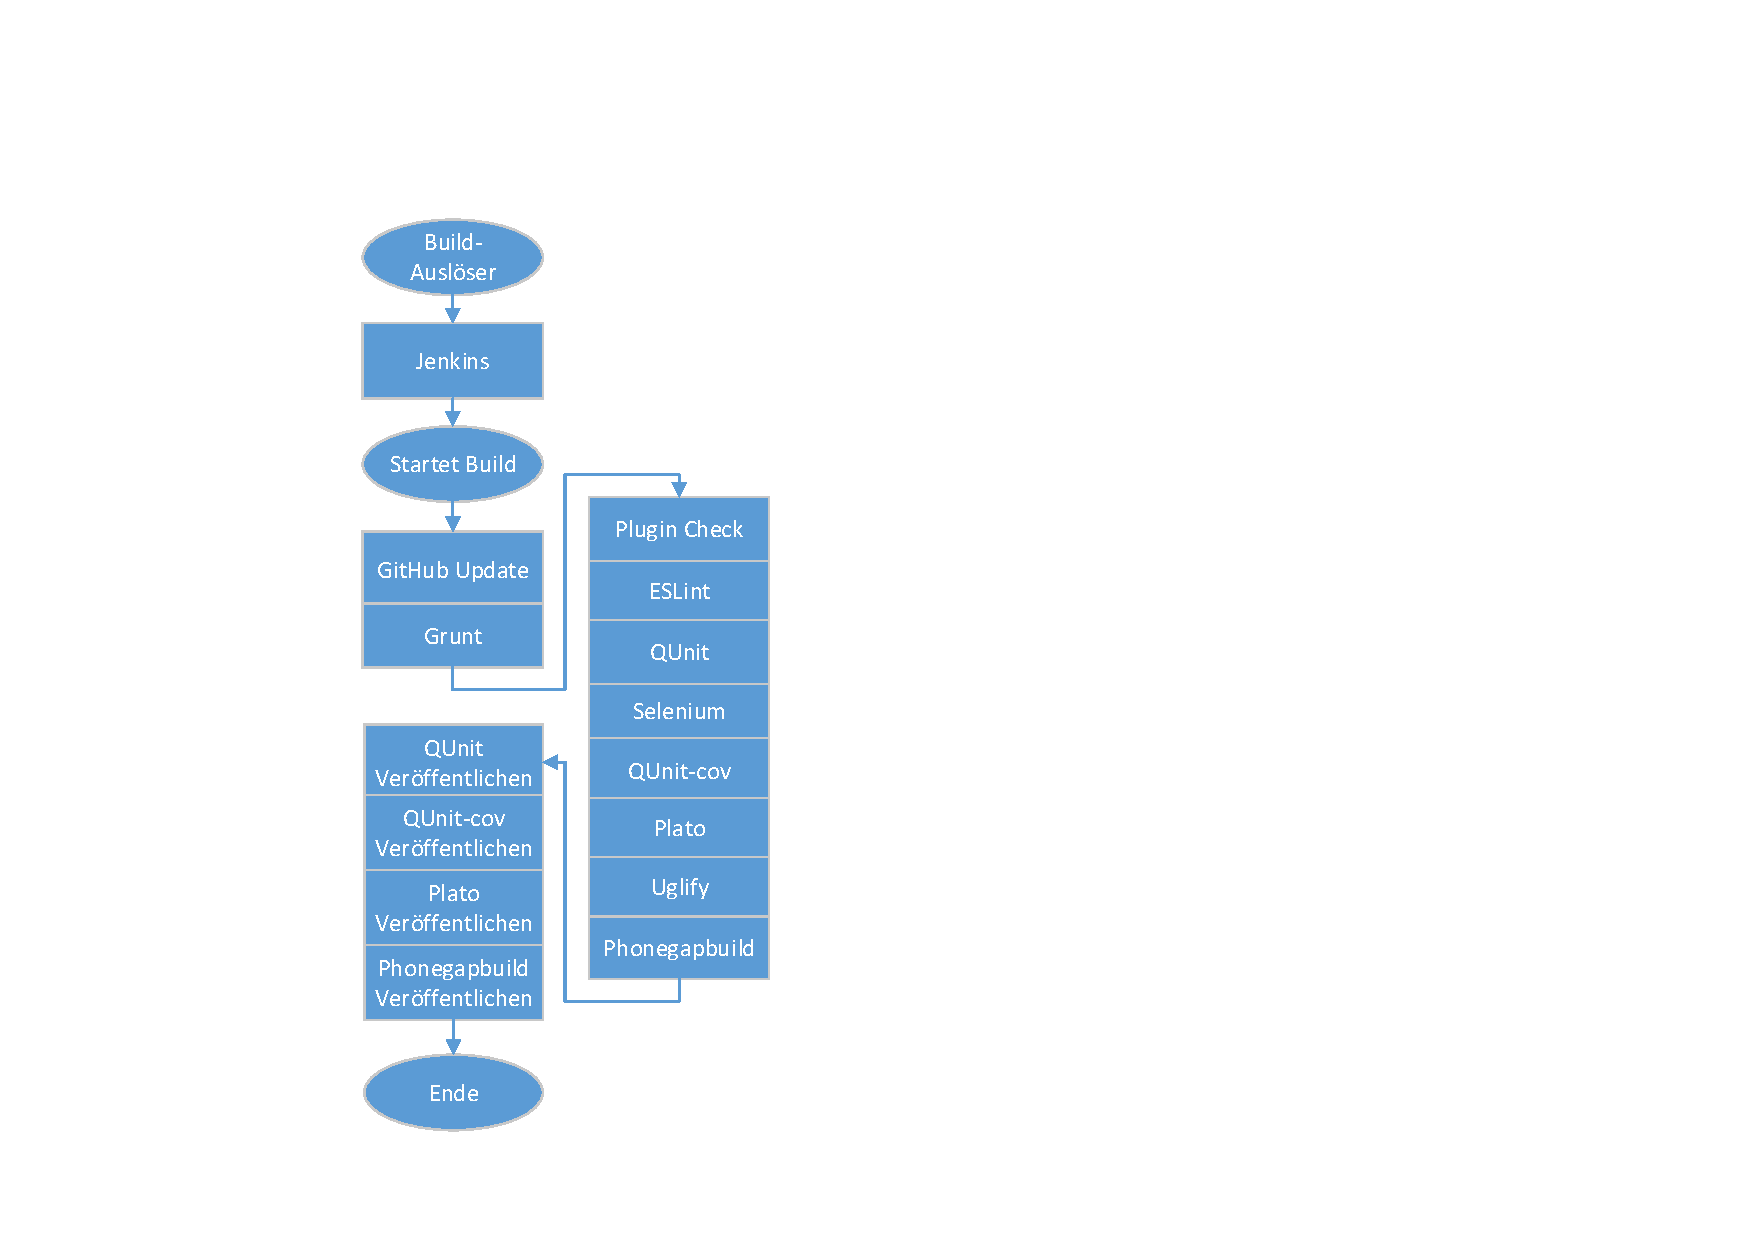
\includegraphics[width=.95\textwidth]{ci-toolchain}
	\caption[Angepasste CI-Toolchain]{Angepasste CI-Toolchain.}
	\label{fig:CI-Toolchain}
\end{figure}

\subsubsection{Projektverwaltung}
Allein die Anzahl der bisher erwähnten JavaScript-Test-Frameworks ist hoch. Für einen kompletten Build-Vorgang fehlen zurzeit sogar noch Tools. Wie in \autoref{fig:CI-Toolchain} gezeigt, muss der Code nach dem Test noch bereinigt, komprimiert und veröffentlicht werden. Diese Aufgaben übernimmt ein JavaScript TaskRunner wie Grunt oder Gulp mit wiederum eigenen Plugins.

Zwischen den genannten Tools und Frameworks bestehen Abhängigkeiten, die ein Paketmanager auflösen sollte \cite{Fain2014}. Im Fall der Entwicklungs- und Testtools übernimmt der node.js-Paketmanager npm diese Aufgabe. Für Frontend-Frameworks wie jQuery oder SAPUI5 steht Bower zur Verfügung.

\subsubsection{Viele kleine Helfer}
Die Übersicht zu \ac{TDD} mit JavaScript zeigt: Es gibt eine große Vielfalt an Frameworks. Diese sind oft klein und erfüllen nur spezielle Aufgaben. Die Mehrheit wird in OpenSource-Communities entwickelt und beeinflusst sich gegenseitig stark. Das Entwicklungstempo ist hoch, und so sind bestehende Best Practices innerhalb weniger Monate oder Jahre hinfällig.

Die Herausforderung während der Implementierung wird in der Auswahl der geeigneten Tools und Frameworks liegen: Welche Teile können aus SAPUI5 übernommen werden, was muss durch externe Module ergänzt werden? Ist die große Modularität des Java-Script-Workflows eine Stärke aus der ein Standard entwickelt werden kann?

\autsection{SAP Mobile}{Mattfeld}
Das UI5 Development Toolkit for HTML5 (SAPUI5) steht im Mittelpunkt der aktuellen SAP-Mobile-Strategie. Als geräteübergreifendes HTML5-Frame\-work soll es schrittweise die SAP GUI und mobile Eigenentwicklungen ablösen. Viele Standardanwendungsfälle werden bereits von den mitgelieferten Fiori Apps auf UI5-Basis abgedeckt. Die ebenfalls neuen Screen Personas sind dagegen nur eine Übergangslösung, um vorhandene Transaktionen vereinfacht darzustellen.

Verfügbar ist UI5 als proprietäres SAPUI5 für SAP-Kunden oder als quelloffenes OpenUI5. Da der Kern beider Versionen identisch ist, sprechen wir im Folgenden nur noch von UI5.

Laut Gartner ist die zugehörige SAP Mobile Platform (SMP) schon jetzt führende Entwicklungs-Plattform für mobile Applikationen \cite{Gartner2014}. Auch die Ankündigung der SAP, den Mainstream Support der SMP 3.0 bis 2020 zu verlängern \cite{Mielke2015}, unterstreicht den Zukunftscharakter dieser Technologie. Bisherige Lessons Learned aus UI5-Projekten zeigen vor allem Potenzial in den Bereichen Entwicklungsumgebung, Test-Entwicklung und -Automatisierung \cite{Thiebes2014}, die wir daher besonders betrachten.

\subsection{UI5-Interna}
Das Framework besteht aus mehreren Bibliotheken: Immer geladen werden \textit{sap.ui.core} und \textit{sap.ui.commons}, das Standard-Bedienelemente beinhaltet. Für unsere App werden wir außerdem \textit{sap.m} nutzen, das seine UI-Elemente dynamisch an die Bildschirmgröße anpasst. Während diese Bibliotheken auch im quelloffenen OpenUI5 vorhanden sind, haben nur zahlende Kunden Zugriff auf \textit{sap.viz} und \textit{sap.makit} zur Diagrammerstellung.

Die Entwicklung von SAPUI5 begann schon 2011, ist jedoch keine vollständige Neuentwicklung. Integriert werden verschiedene Open-Source-Framworks wie jQuery, jQuery Mobile, data.js, QUnit und Sinon.JS -- Kombiniert ergeben sie ein JavaScript-Framework, dass sich auch für umfangreiche Unternehmensanwendungen eignet und durch jQuery-Plugins oder eigene Steuerelemente erweitert werden kann.

Im Unterschied zu jQuery Mobile als Einzelframework unterstützt es Modularisierung, Internationalisierung, Routing, Testbarkeit und vieles mehr. Es befindet sich damit auf einer Ebene mit anderen Enterprise Frameworks wie Sencha Ext JS inkl. Sencha Touch oder AngularJS, die ähnliche Ansätze verfolgen.

UI5-Apps basieren auf der \ac{MVC}-Architektur. Die Anwendungslogik wird in den Browser verlagert. Der zuständige Controller ist grundsätzlich in JavaScript implementiert. Views werden dynamisch ebenfalls per JavaScript erzeugt oder statisch als XML, HTML oder JSON definiert. Das Model bezieht die App über \ac{REST}-Services. 


\subsection{Architekturen}
\label{sec:architekturen}
Das SAP Gateway liefert entsprechende OData-Services nach dem REST-Prinzip:

\begin{itemize}
	\item Zustandslos -- Operationen sind in sich abgeschlossen
	\item Übertragung im XML-Format
	\item Navigationseigenschaften -- \zB Verlinkung vom Kunden zum Projekt
	\item URL-adressierbare Objekte -- \zB \textit{http://\dots/Kunde(3)/Projekt(1)}
	\item Operationsbasiert -- \zB \textit{GET, POST, PUT, DELETE, \dots}
\end{itemize}
Diese Services lassen sich auf Basis verschiedener Quellen implementieren und sind insgesamt leichter handhabbar als ihre Vorgänger SOAP/WSDL. \autoref{sec:neues_backend} zeigt die wichtigsten Möglichkeiten.

Die für mobile Geschäftsanwendungen oft geforderte Offline-Fähigkeit ergibt sich allerdings erst im Zusammenspiel mit der \textit{SAP Mobile Platform 3.0} oder ihrem Cloud-Pendant \textit{HANA Cloud Platform mobile services} auf Basis der ehemaligen Sybase Unwired Platform. Single Sign-on (SSO), Push-Benachrichtigungen und Fernzugriff ohne VPN sind weitere Zusatzfunktionen beider Lösungen. 

Daraus folgen mindestens fünf Deployment- und App-Architekturen, die sich vor allem in den nutzbaren Business- und Geräte-Funktionen unterscheiden:
\begin{enumerate}
	\item Web
	\item Fiori-Launchpad-Integration
	\item Zugriff über Fiori Client
	\item Hybrid-App
	\item Angepasster Fiori Client
\end{enumerate}
Methode 1 eignet sich für alle Arten von UI5-Apps. Die Veröffentlichung kann auf jedem beliebigen Webserver erfolgen. Ein SAP-Bezug ist nicht nötig. Allerdings werden keine weiteren Business- oder Geräte-Funktionen unterstützt.

\begin{figure}[b]
	\centering
	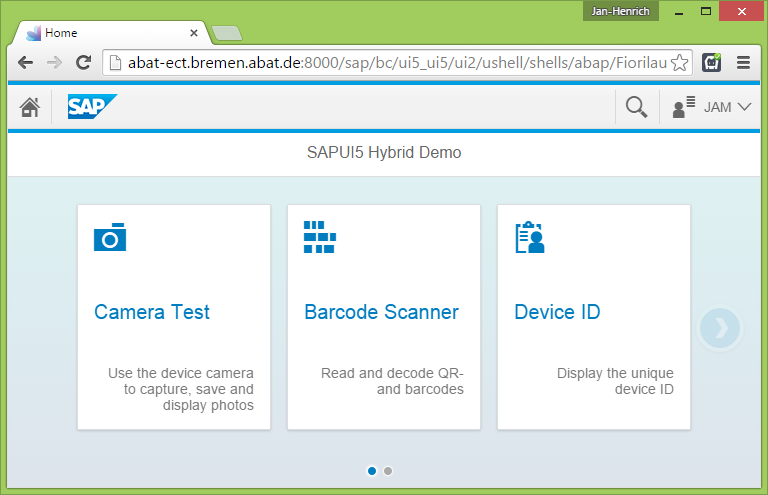
\includegraphics[width=.85\textwidth]{SAPUI5_Hybrid_Fiori2} 
	\caption[UI5-Eigenentwicklung im Fiori Launchpad]{UI5-Eigenentwicklung im Fiori Launchpad.}
	\label{fig:SAPUI5_Hybrid_Fiori2}
\end{figure}

Zur Fiori-Launchpad-Integration ist eine bestimmte App-Struktur und Modularisierung nötig. Die App wird normalerweise über ein ABAP-Reposit\-ory veröffentlicht. Vorteile sind die SSO-Möglichkeit und ein einheitliches Benutzererlebnis durch die Integration in Fiori wie in \autoref{fig:SAPUI5_Hybrid_Fiori2}.

Der Fiori Client ist für iOS und Android verfügbar. Wird das Launchpad durch ihn aufgerufen, speichert er Zugangsdaten und App-Inhalte im Cache: Die Performance wird verbessert. Weitere Gerätefunktionen sind zur Zeit nicht nutzbar.

UI5-Apps lassen sich beliebig in eigene Hybrid-Apps auf Cordova-Basis integrieren, um native Gerätefunktionen wie Kamera oder GPS aufzurufen. Geschäftsfunktionen und der Zugriff auf die SAP-Infrastruktur gelingt aber nur mit einem angepassten Fiori Client. Der Client-Quellcode ist als Teil des Mobile Platform SDKs verfügbar. Zusammen mit den sogenannten Kapsel Plugins (Cordova) ist das der einzige Weg, um die Offline- und Push-Funktionen der Mobile Platform (SMP) nutzbar zu machen.

\subsection{Open-Source-Initiative als Chance}
\label{sec:os_chance}
Historische Entwicklungen auf Basis der SAP-eigenen Programmiersprache ABAP
(Advanced Business Application Programming) lassen sich nur schwer in einem
CI-Prozess automatisieren: Die entsprechenden Werkzeuge z.\,B. zum
ABAP-Unit-Test \cite{Majer2009} oder zur Testfallerstellung (eCATT) liegen vor,
lassen sich aber nur schwer einbinden. Eine weitere Rolle spielt die
grundsätzliche ABAP-Entwicklung im System selbst -- Eine CI-Interaktion von
außen gestaltet sich schwierig.

Deutlich mehr Möglichkeiten ergeben sich bei SAP-Entwicklungen auf Java-Basis:
Hier steht die SAP NetWeaver Development Infrastructure (NWDI) zur Verfügung
\cite{Chan2011}.
Alle CI-relevanten Tasks sind vorhanden und lassen sich automatisieren.
NWDI ist allerdings proprietär und eignet sich nicht zur Entwicklung mit anderen
Plattformen als Java EE.

Eine komplette Kehrtwende ergibt sich nun nach der Einführung von SAPUI5 als
neue SAP-Mobilplattform: Sie ist auch ohne SAP-Backend lauffähig und basiert auf
dem weit verbreiteten JavaScript-Framework jQuery \cite{Antolovic2014}.
Zusätzlich sind große Teile des Quellcodes unter dem Namen OpenUI5 auf GitHub
veröffentlicht worden -- inklusive Buildkonfiguration und ausführlicher
Dokumentation \cite{SAP2014_1}. Sie geben einen guten Einblick in den
SAP-internen Workflow. 

In der Bachelorarbeit wird untersucht, welche Teile für
eigene Projekte übernommen werden können. Wo sind größere Anpassungen und
Erweiterungen notwendig? Testbarkeit spielte bei der Entwicklung des Frameworks offenbar eine größere
Rolle als früher: Frei verfügbar sind bereits der QUnit-Aufsatz OPA5 (One-Page
Acceptance tests for UI5) und ein Mock-Server zur Emulation von OData-Services
\cite{BoennenDreesFischerHeinzStrothmann2014}.

\subsubsection{Gute Voraussetzungen} 
Folgende Aspekte begünstigen den Aufbau einer SAPUI5-CI-Toolchain mit Jenkins (siehe \nameref{fig:CI-Toolchain}):
\begin{quote}
	\begin{enumerate}
		\item Bewährte Basistechnologien
		\item Open-Source-Vorstoß
		\item Testorientierung
		\item Wachsende Community
	\end{enumerate}
\end{quote}


\autsection{Neues Backend: SAP Gateway}{Azimi}
\label{sec:neues_backend}
Das SAP Gateway wurde im Mai 2011 auf den Markt gebracht, um die Reichweite von SAP-Geschäftsanwendungen zu erhöhen. 
Dazu bietet das Gateway eine offene, REST-basierte Schnittstelle, um einen einfachen Zugriff auf SAP-Systeme zu ermöglichen, siehe \autoref{fig:GatewayArchitektur}.
Das offene Protokoll OData wird verwendet, da es viel genutzt, bekannt und leicht zu lernen ist. Damit soll die SAP-Welt jedem Entwickler zugänglich sein, der OData versteht, da kein spezielles SAP-Fachwissen mehr nötig ist, um eine Oberfläche für Anwendungen und den Zugriff auf SAP-Daten zu entwickeln.

Durch die Bereitstellung der OData-Schnittstelle müssen der Backend-Entwickler und der Frontend-Entwickler nicht wissen, was der jeweils andere im Detail programmiert. Eine klare Definition der benötigten Schnittstellen ist allerdings zwingend notwendig und erleichtert die gesamte Entwicklung \cite[S.\ 31-45]{BoennenDreesFischerHeinzStrothmann2014}.

\begin{figure}
	\centering
	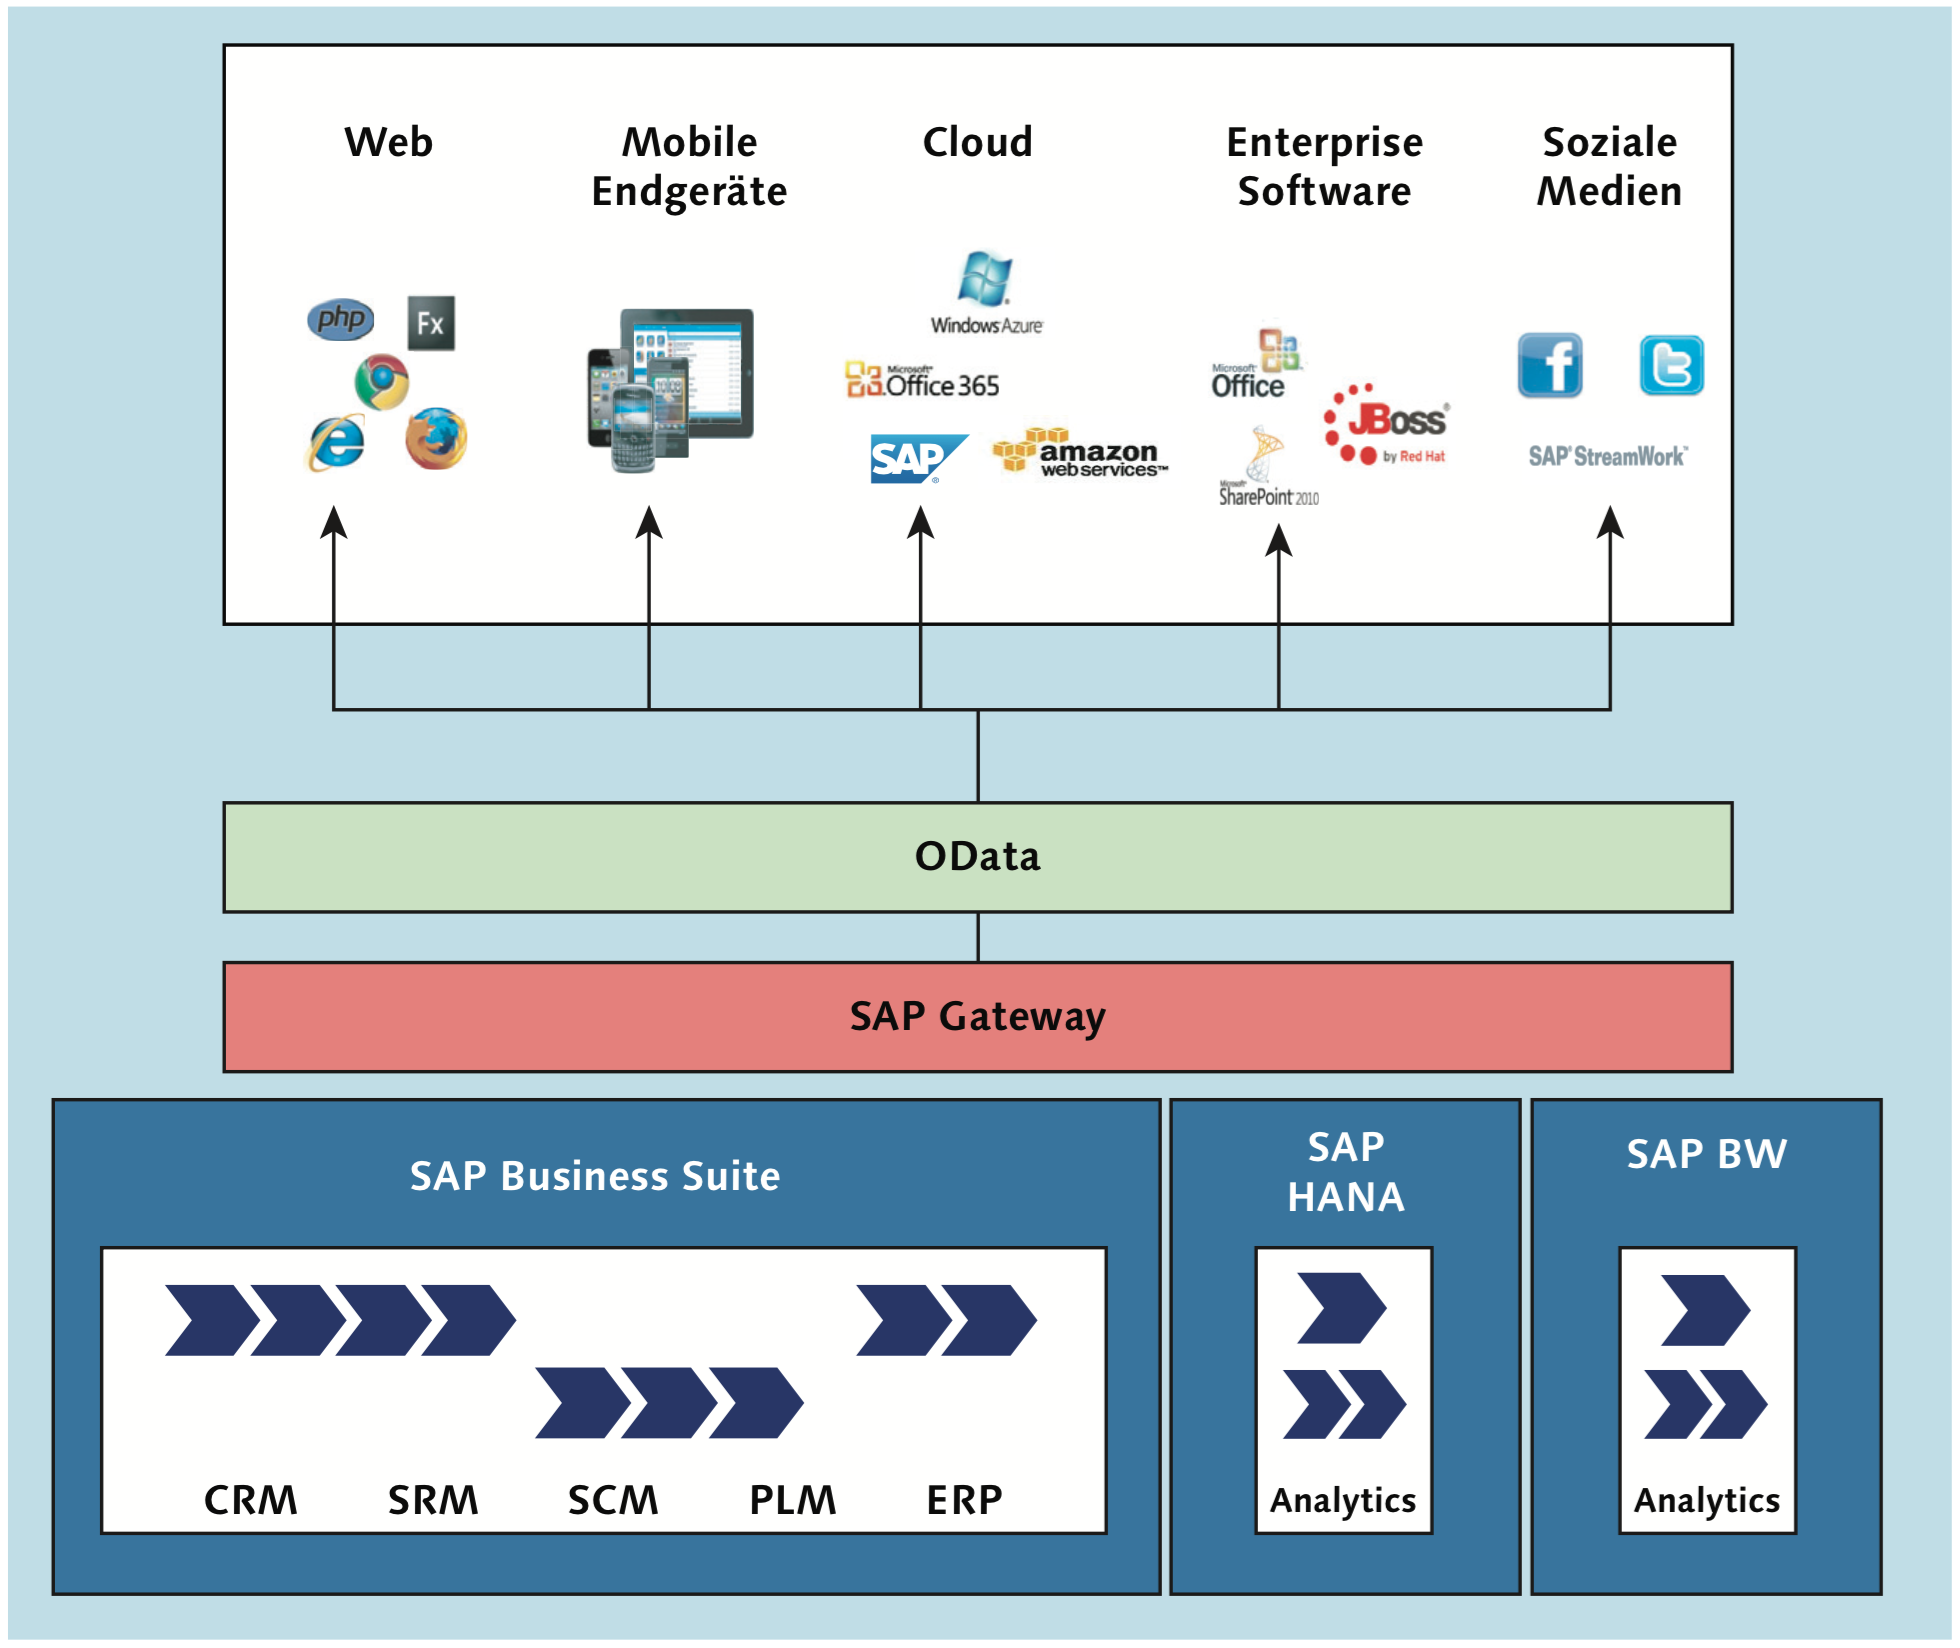
\includegraphics[width=.95\textwidth]{Gateway_architektur_page45} 
	\caption[SAP-Gateway-Integrationsmodell]{SAP-Gateway-Integrationsmodell aus \cite[S.\ 45]{BoennenDreesFischerHeinzStrothmann2014}.}
	\label{fig:GatewayArchitektur}
\end{figure}

\subsection{Best Practices}
Um möglichst hochwertige Anwendungen mit Hilfe von OData-Services zu entwickeln, empfiehlt SAP folgende Best Practices zu beachten\cite[S.\ 561-563]{BoennenDreesFischerHeinzStrothmann2014}: 
\begin{itemize} 
	\item Kommunikation zwischen den Entwicklungsteams zur genauen Spezifikation der Schnittstellen.
	\item Frühzeitiger Entwicklungsbeginn des OData-Services, damit dem Front\-end-Entwicklerteam möglichst früh ein konsumierbarer Service zur Verfügung steht. 
	\item Gruppierung der Services in Module, sodass die Anwendung auf bereits vollständig entwickelte Teil-Services zugreifen kann. 
	\item Gründliches Testen der vollständig entwickelten OData-Services mit Hilfe von Test-Tools, sowie zusätzliche Tests mit der entwickelten Anwendung. 
	\item Frühzeitiges Testen in der Produktivumgebung.
	\item Nutzen der Query-Option \textit{sap-ds-debug=true} im Browser.
 \end{itemize}

\subsection{Deployment-Optionen}
Für das Deployment des SAP Gateways stehen verschiedene Optionen zur Verfügung. Diese werden nachfolgend beschrieben.

\subsubsection{Eingebettetes Deployment}

Bei dieser Variante des Deployments werden alle Komponenten des SAP Gateways auf dem SAP-Backend-System installiert. Ab SAP NetWeaver\,7.40 ist das Gateway Bestandteil der Standardinstallation. Hauptvorteil ist die Reduzierung der Laufzeit um einen Remote Call: Der Service wird direkt auf dem Backend registriert. Der Nachteil an dieser Variante ist, dass das SAP Gateway für jedes Backend separat konfiguriert werden muss.

Zudem rät SAP davon ab, SAP-Backend-Systeme mit eingebettetem Gateway als Hub-System für andere Backends zu verwenden. Abhängigkeiten im Aktualisierungsprozess können ein Hub-Update bei bereits aktualisiertem Backend-System verhindern \cite[S.\ 52-54]{BoennenDreesFischerHeinzStrothmann2014}.

\subsubsection{Hub-Deployment mit Entwicklung auf dem SAP-Backend}

Die Gateway-Kernkomponenten werden auf einem zusätzlichen SAP-Gate\-way-Hub-System installiert. Zusätzlich muss auf dem SAP-Backend-System die Business-Enablement-Provisioning-Komponente (\textit{IW\_BEP}) installiert werden. Bei dieser Variante wird der Service auf dem Backend-System entwickelt und veröffentlicht (deployt). Der Service wird anschließend auf dem Gateway Hub registriert. Beim Hub-Deployment ist es möglich, mehrere SAP-Backends mit dem Gateway zu verbinden. Zudem gibt es hier keinen direkten Zugriff auf das SAP-Backend-System \cite[S.\ 54]{BoennenDreesFischerHeinzStrothmann2014}.

\subsubsection{Hub-Deployment mit Entwicklung auf dem Hub}

Alle Komponenten des SAP Gateways werden auf dem Hub-System installiert. Diese Variante wird beispielsweise bei eingeschränktem Zugriff auf das Backend-System eingesetzt, falls eine Entwicklung auf diesem nicht möglich ist. Zwingend ist diese Variante bei Release-Ständen unter SAP NetWeaver\,7.40, dort ist eine Installation von \textit{IW\_BEP}  auf dem Backend nicht erlaubt. 

Die Entwicklung des Services findet auf dem Hub-System statt. Vorteil: Das SAP-Backend-System wird nicht modifiziert. Allerdings muss bei der Entwicklung auf eine bereits vorhandene Schnittstelle wie \zB einen \ac{RFC} oder ein \ac{BAPI} zurückgegriffen werden, die das Backend bereitstellt \cite[S.\ 55]{BoennenDreesFischerHeinzStrothmann2014}.


\subsection{OData und REST}
Das \ac{OData} ist ein REST-basiertes Datenzugriffsprotokoll, welches unter der \ac{OSP} herausgegeben wurde und auf verbreiteten Standards wie Atom Pub, XML und JSON aufbaut \cite[S.\ 69-70]{BoennenDreesFischerHeinzStrothmann2014}.
Um eine \ac{REST}-konforme Architektur einzuhalten müssen folgende Eigenschaften erfüllt werden \cite[S.\ 65-66]{BoennenDreesFischerHeinzStrothmann2014}:

	\begin{enumerate}
	\item \textbf{Client-Server-Architektur} --
	Client und Server werden von einer einheitlichen Schnittstelle getrennt.
	\item \textbf{Zustandslosigkeit} --
	Es werden keine Daten zu den einzelnen Abfragen gespeichert. Daher muss jede Abfrage alle benötigten Informationen beinhalten.
	\item \textbf{Pufferbarkeit} --
	Die Antworten des Servers müssen spezifizieren, wie lange Daten gespeichert werden dürfen, damit keine veralteten oder falschen Daten verwendet werden.
	\item \textbf{Mehrschichtigkeit} --
	Der Client weiß nicht, ob er direkt mit dem Backend oder nur mit einem Server in der Mitte verbunden ist.
	\item \textbf{Einheitliche Schnittstelle} -- Die Ressourcen werden nach einem einheitlichen Verfahren identifiziert, wie \zB Name, Pfad oder Primärschlüssel. Abfrage und Manipulation von Ressourcen geschehen nach einem einheitlichen Verfahren.
	\end{enumerate}
Durch OData werden dem Konsumenten definierte Schnittstellen für verschiedene Datenquellen zur Verfügung gestellt und soll so die Zusammenarbeit zwischen verschiedenen Plattformen ermöglichen \cite[S.\ 69-70]{BoennenDreesFischerHeinzStrothmann2014}.

\subsubsection{Datenmodell}
Für den OData-Service muss ein \ac{EDM} definiert werden, welches über das Metadaten-Dokument für Clients zum Abruf  bereit steht. Im \ac{EDM} werden die einzelnen Entitäten, Entitätstypen und ihre Attribute definiert. Des Weiteren werden die Kardinalitäten zwischen den einzelnen Entitäten über Assoziationen festgelegt, sodass über Navigationsattribute zwischen den einzelnen Entitäten navigiert werden kann \cite[S.\ 72-73]{BoennenDreesFischerHeinzStrothmann2014}.


\subsubsection{Servicedokumente}

Im Servicedokument (siehe Listing \ref{lst:Servicedokument}) werden alle Entitätsmengen, welchen immer ein Entitätstyp zugrunde liegt, eines Services angezeigt. Zudem werden SAP-spezifische Metainformationen angezeigt, welche unter anderem beschreiben, ob die Entitätsmengen das Hinzufügen, Ändern oder Entfernen von Einträgen oder das erlauben. Erreichbar ist das Servicedokument über den Aufruf des Services ohne zusätzliche Parameter \cite[S.\ 77-81]{BoennenDreesFischerHeinzStrothmann2014}. Die URI zu einem Servicedokument könnte Beispielsweise so aussehen: \\\textit{http://host:port/sap/opu/odata/sap/Z\_ZAV\_SCRUM\_SRV/}\\

\begin{listing}[h]
	\inputminted{xml}{src/servicedokument-short.xml}
	\caption{Servicedokument Z\_ZAV\_SCRUM\_SRV}
	\label{lst:Servicedokument}
\end{listing}

Im Service-Metadokument (siehe Listing \ref{lst:Metadata}) sind die gesamten Metainformationen, inklusive Datenmodell, Entitätstypen, Entitätsmengen, Assoziationen und Navigationseigenschaften des Services enthalten. Dadurch kennt der Zugreifende alle Informationen über Struktur, Ressourcen und Verknüpfungen \cite[S.\ 81-82]{BoennenDreesFischerHeinzStrothmann2014}. Aufgerufen wird das Service-Metadokument über den zusätzlichen Parameter \textit{\$metadata} wie im folgendem Beispiel: 
\\\textit{http://host:port/sap/opu/odata/sap/Z\_ZAV\_SCRUM\_SRV/\$metadata}

\begin{listing}[h]
	\inputminted{xml}{src/metadata.xml}
	\caption{Metadaten Z\_ZAV\_SCRUM\_SRV}
	\label{lst:Metadata}
\end{listing}